\documentclass[11pt]{article}
\usepackage{fullpage}
\usepackage{latexsym}
\usepackage{verbatim}
\usepackage{code,proof,amsthm,amssymb, amsmath}
\usepackage{ifthen}
\usepackage{graphics}
\usepackage{mathpartir}

%% Question macros
\newcounter{question}[section]
\newcounter{extracredit}[section]
\newcounter{totalPoints}
\setcounter{totalPoints}{0}
\newcommand{\question}[1]
{
\bigskip
\addtocounter{question}{1}
\addtocounter{totalPoints}{#1}
\noindent
{\textbf{Task \thesection.\thequestion}}[#1 points]:


}
\newcommand{\ecquestion}
{
\bigskip
\addtocounter{extracredit}{1}
\noindent
\textbf{Extra Credit \thesection.\theextracredit}:}


\newcounter{taskcounter}
\newcounter{taskPercentCounter}
\newcounter{taskcounterSection}
\setcounter{taskcounter}{1}
\setcounter{taskPercentCounter}{0}
\setcounter{taskcounterSection}{\value{section}}
\newcommand{\mayresettaskcounter}{\ifthenelse{\value{taskcounterSection} < \value{section}}
{\setcounter{taskcounterSection}{\value{section}}\setcounter{taskcounter}{1}}
{}}

% Solution-only - uses an "input" so that it's still safe to publish the problem set file
\definecolor{solutioncolor}{rgb}{0.0, 0.0, 0.5}
\newcommand{\solution}[1]
  {\ifthenelse{\equal{\issolution}{true}}
  {\begin{quote}
    \addtocounter{taskcounter}{-1}
    \fbox{\textcolor{solutioncolor}{\bf Solution \arabic{section}.\arabic{taskcounter}}}
    \addtocounter{taskcounter}{1}
    \textcolor{solutioncolor}{\input{./solution/#1}}
  \end{quote}}
  {}}

\newcommand{\qbox}{\fbox{???}}

\setcounter{taskcounter}{1}
\setcounter{taskPercentCounter}{0}
%\setcounter{taskcounterSection}{\value{section}}

\newcommand{\ttt}[1]{\texttt{#1}}

%% part of a problem
\newcommand{\task}[1]
  {\bigskip \noindent {\bf Task\addtocounter{taskPercentCounter}{#1} \arabic{taskcounter}\addtocounter{taskcounter}{1}} (#1\%).}

\newcommand{\ectask}
  {\bigskip \noindent {\bf Task \arabic{section}.\arabic{taskcounter}\addtocounter{taskcounter}{1}} (Extra Credit).}

\newcommand{\val}[1]{#1~\textsf{val}}
\newcommand{\num}[1]{\texttt{num}[#1]}
\newcommand{\str}[1]{\texttt{str}[#1]}
\newcommand{\plus}[2]{\texttt{plus}(#1; #2)}
\newcommand{\mult}[2]{\texttt{times}(#1; #2)}
\newcommand{\cat}[2]{\texttt{cat}(#1; #2)}
\newcommand{\len}[1]{\texttt{len}(#1)}
\newcommand{\abst}[2]{#1.#2}
\newcommand{\letbind}[3]{\texttt{let}(#1; \abst{#2}{#3})}
\newcommand{\steps}[2]{#1 \mapsto #2}
\newcommand{\subst}[3]{[#1/#2]#3}
\newcommand{\err}[1]{#1~\textsf{err}}

\newcommand{\proves}{\vdash}
\newcommand{\hasType}[2]{#1 : #2}
\newcommand{\typeJ}[3]{#1 \proves \hasType{#2}{#3}}
\newcommand{\ctx}{\Gamma}
\newcommand{\emptyCtx}{\emptyset}
\newcommand{\xCtx}[2]{\ctx, \hasType{#1}{#2}}
\newcommand{\typeJC}[2]{\typeJ{\ctx}{#1}{#2}}
\newcommand{\numt}{\texttt{num}}
\newcommand{\strt}{\texttt{str}}

\newcommand{\laz}[1]{\left[ #1 \right]}


\title{Assignment \#1: \\
        Abstract Binding Trees, Dynamics and Statics}

\author{15-312: Principles of Programming Languages}
% put together by Cyrus Omar and Shayak Sen, based on assignments from S10 and S09
\date{Out: Tuesday, January 21st, 2014\\
      Due: Tuesday, February 4th, 2014 1:29PM}

\begin{document}
\maketitle
\section*{Introduction}

This assignment consists of two major parts. The first part involves building up an infrastructure to represent and manipulate abstract syntax with binding. The second part will be to implement the calculator language we have been discussing in class, also introduced in Ch. 4 of PFPL. You will begin by implementing a version without a static type system, then you will implement a statically typed version to see the key differences between these approaches.

There is quite a bit of code to understand and implement in this assignment. Start early.

\subsection{Submission}
We will collect {\it exactly} the following files:
\begin{quote}
\begin{verbatim}
/afs/andrew/course/15/312/handin/<yourandrewid>/assn1/assn1.pdf
/afs/andrew/course/15/312/handin/<yourandrewid>/assn1/abt.sml
/afs/andrew/course/15/312/handin/<yourandrewid>/assn1/abt-util.sml
/afs/andrew/course/15/312/handin/<yourandrewid>/assn1/termops.sml
/afs/andrew/course/15/312/handin/<yourandrewid>/assn1/checkeddynamics.sml
/afs/andrew/course/15/312/handin/<yourandrewid>/assn1/typechecker.sml
/afs/andrew/course/15/312/handin/<yourandrewid>/assn1/uncheckeddynamics.sml
\end{verbatim}
\end{quote}
Make sure that your files have the right names (especially
\verb'assn1.pdf'!) and are in the correct directory.

\section{Abstract Binding Trees}
Abstract binding trees, introduced in Section 1.2 of PFPL, are used to represent the abstract syntax of languages with variables and binding. We will begin by building a generalized infrastructure to support abstract binding trees for any such language.

\subsection{Variables}

A variable in an abstract binding tree (ABT) is a placeholder for a fixed, but unspecified ABT. A key idea is the notion of a \emph{new} or \emph{fresh variable} -- one that has not been seen before in some given context. To work with variables, we introduce the \verb|VARIABLE| signature, reproduced below.

\verbatiminput{../code/var-sig.sml}

There are several ways to guarantee uniqueness, but one simple way is to just ignore the context and make sure every freshly generated variable is globally unique.  We provide such an implementation that satisfies this signature for you in the \verb|Var| module. You can read the source code in \verb|var.sml| if you'd like, but you don't have to (that's the magic of signatures!)

\subsection{Operators}

In PFPL, we specify
every language as a collection of operators. Each operator $o$
has an arity $\mathsf{ar}(o) = (n_1, \ldots, n_k)$, where the length $k$
gives the number of arguments the operator takes and each $n_i$ specifies the \emph{valence}
of the $i$-th argument, which is the number of variables bound
by that argument.

We will work with operators via a signature, \verb|OPERATOR|.

\verbatiminput{../code/oper.sig}

We will ask you to give an implementation of this signature in Section 2 below. But for now, what we're going to do is develop an
implementation of ABTs that is parametric in the \verb|OPERATOR| signature,
so that you can instantiate it in different ways to automatically construct the syntax
for the different languages we will study in this course.

\subsection{Abstract Binding Trees}

Now, we can introduce the signature of abstract binding
trees. This is a version
of an interface to syntax that has been developed here at CMU over
numerous compiler development efforts, and is designed to help
users avoid running into some very common errors.

\verbatiminput{../code/abt.sig}

The first two fields of the \texttt{ABT} signature simply say
that it has two sub-modules, \texttt{Variable} and \texttt{Operator},
which are the variable and operator implementations for the particular
language syntax being implemented.

Then, we introduce an abstract type \texttt{t} for the actual internal
represention of an abstract binding tree.
However, there are no simple functions that construct values of
type \texttt{t} directly. Instead, access to the representation type \texttt{t}
is mediated by a \emph{view}, which is a \textbf{non-recursive} datatype \texttt{'a
  view}, and a pair of functions \texttt{into} and \texttt{out}.
The idea behind a view is that it is a type whose values represent a
one-step unfolding of a value of the abstract type \texttt{t}. The function
\texttt{out} does this one-step unfolding of an ABT to create a view, and \texttt{into} puts a
view back together into an ABT.

More specifically, the function \texttt{out} has type \texttt{t -> t view}. This means it
takes an ABT value, and deconstructs it as follows:

%To make the code look clean, we use the \texttt{infix} operator to make
%$\mathtt{\backslash}$ and \texttt{\$} infix constructors.

\begin{itemize}
\item Suppose that the term \texttt{e} of type \texttt{t}
  represents the abstract binding tree $x$. Then, a call \texttt{out
    e} would return \texttt{` x}, where the value
  \texttt{x}, of type \texttt{Variable.t}, represents the variable $x$.

\item Likewise, suppose a term \texttt{e} represents an abstract
  binding tree $f(e_1, \ldots, e_n)$, where $f$ is an operator.
  Then a call \texttt{out e} should return \texttt{\$ (f, es)}, where \texttt{f} is a term of
  type \texttt{Operator.t} representing $f$, and \texttt{es} is a term
  of type \texttt{t list}, whose elements represent the
  ABTs of each $e_i$ in the argument sequence $(e_1, \ldots, e_n)$ -- but \emph{not} views to them. This is what we mean by a one-step unfolding.

\item Finally, if a term \texttt{e} represents an abstract binding
  tree $x.e'$, then the call \texttt{out e} will return \verb|\ (y, e'')|
  where \verb|y| represents a fresh variable $y$ and \verb|e''|
  represents the ABT $[y \leftrightarrow x]e'$, where $[y \leftrightarrow x]e$ means
  ``substitute \emph{free} occurrences of $x$ in $e$ with $y$''.

  In other words, the \texttt{out} operation renames the variable bound by
  an abstractor whenever it unpacks it! This is one of the essential
  features of this interface, and implementing this correctly will save you
  many hours tracing down strange $\alpha$-conversion issues.
\end{itemize}

The function \texttt{into} has type \texttt{t view -> t}, and folds
a one-step unfolding (that is, a view) back into an ABT term.

\begin{itemize}
\item Suppose \texttt{x} is a term of type \texttt{Variable.t}, which
  represents the variable $x$. Then \texttt{into (` x)} will return
  the abstract binding tree corresponding to the variable occurence $x$.

\item If \texttt{x} is a term of type \texttt{Variable.t}, which
  represents the variable $x$; and \texttt{e} is a term of type
  \texttt{t} representing the ABT $e$, then \verb|into (\ (x, e))|
  will return a term representing the abstractor $x.e$.

\item If \texttt{f} is a term of type \texttt{Operator.t}, representing
   the operator $f$, and \texttt{es} is a term of type \texttt{t list},
   representing the sequence $(e_1, \ldots, e_n)$. Then
   \texttt{into (\$ (f, es))} will return a term representing
   $f(e_1, \ldots, e_n)$ if the arity of $f$ matches the
   sequence. Otherwise, it will raise the exception \texttt{Malformed}.
\end{itemize}


However, \texttt{into} is not quite the inverse of \texttt{out}. If
\texttt{e} is a term of type \texttt{t}, then \texttt{e} and
\texttt{into(out(e))} will not in general represent equal ABTs -- but
they will, however, always represent $\alpha$-equivalent ABTs!
We can test $\alpha$-equivalence with the \verb|aequiv| function,
which returns true if its two arguments are $\alpha$-equivalent, and
false otherwise. This means that \texttt{aequiv(into(out(e)), e)}
is always true.

Finally, we have a convenience function \texttt{map} in this
interface. Given a function \texttt{f} of type \texttt{'a -> 'b}, it
takes an \texttt{'a view} and produces a \texttt{'b view} by applying
it to each subterm of type \texttt{'a}, and leaving all of the other
subterms and constructors unchanged.

\task{5} Suppose \texttt{v} has type \texttt{t view}. Will \texttt{out(into(v))} be equal to \texttt{v}? Explain why or why not.

Think carefully about what effect the renaming \texttt{out} can
perform before answering this question.

\solution{q1a.tex}

\subsection{Implementing ABTs}

One of the inconveniences of using a straightforward representation
of ABTs is that $\alpha$-equivalent terms can have
multiple representations, so implementing \verb|aequiv| and other helper functions becomes tricky. We will look at a more sophisticated representation,
called \emph{locally nameless form}, which avoids this problem, so
that each $\alpha$-equivalence class is represented with a single
data value, and thus $\alpha$-equivalence can be tested for with a
simple structural traversal.

The basic idea is to observe that variables in an abstract binding
tree serve two roles. First, they can appear free in a ABT -- that is,
they can be a \emph{name} for a hypothesis in some hypothetical
context. Second, they can be a bound variable, in which case the variable
occurences \emph{refer back} to the location of the binding
abstraction. For example, in the ML term

\begin{verbatim}
  let x = 5 in let y = 3 in (x, x + y + C)
\end{verbatim}

The bound variable \texttt{x} refers back to the outermost binding,
and the bound variable \texttt{y} refers back to the second
binding. The variable \verb|C| is a free variable. The only reason we need the names of the bound variables is to distinguish one
abstraction site from another -- the names themselves are
irrelevant from a semantic point-of-view. (This is just another way of saying that we want to
identify terms up to $\alpha$-equivalence, of course.)

In a locally nameless representation, we distinguish these two roles
in our data structure, in order to make $\alpha$-equivalence
implementable as structural equality on terms.
The trick in this representation is to exploit a structural invariant
of binding trees. First, binding trees are \emph{trees} -- they have
no cycles in them. Second, in any abstraction $x.e$, the only
occurences of $x$ are within $e$.
As a result of these two facts, we have a \emph{unique} path from an
abstractor to each occurence of the variable it binds. Furthermore,
since we're only interested in the binder sites, we can compress this
path to a single number, which tells us how many binders we have to
hop over before we reach the one we're interested in.

Consider the following diagram of the binding tree $x. A(x, y.
B(z.x, y, z, w. y))$, in which $A$ and $B$ are operator names.

\ \\
\ \\

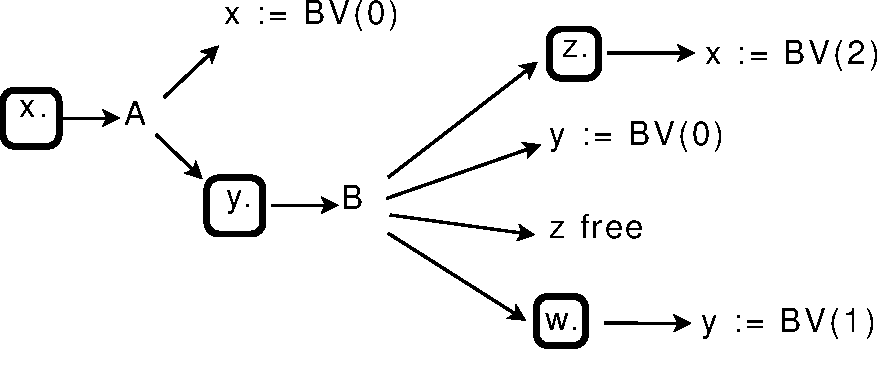
\includegraphics{Diagram1.pdf}

We've put a box around every abstraction, and labelled each bound variable
with its bound variable number. We can calculate the bound variable number
by looking at each path from an abstraction to its use sites, and count
the number of abstractions crossed along the way:

\newcommand{\boxabs}[1]{\mbox{\fbox{${#1}.$}}}
\ \\

\begin{tabular}{l|c}
 Path & Variable \# \\ \hline

$\boxabs{x} \to A \to x$ & 0 \\
$\boxabs{x} \to A \to \boxabs{y} \to B \to \boxabs{z} \to x$ & 2 \\
$\boxabs{y} \to B \to y$ & 0 \\
$\boxabs{y} \to B \to \boxabs{w} \to y$ & 1 \\
\end{tabular}

\ \\

An important fact to notice about these paths is that even for the
same binder, each occurrence of its bound variable can have a \emph{different}
bound variable number, depending on the number of abstractions we
crossed over to reach that variable occurrence.

\task{20} You will need to implement the structure Abt in file \texttt{abt.sml},
implementing ABTs with a locally nameless representation:

\verbatiminput{../code/abt.sml}

\emph{Hint:} When implementing this structure, you will find it
helpful to define two functions \texttt{bind} and \texttt{unbind}.

\begin{itemize}
\item \texttt{bind} should take a term $e$ and a free variable $x$,
and return a new term corresponding to $x.\;e$.

\item \texttt{unbind} should take a term $x.\;e$, and return a
variable $x'$, and a term corresponding to $[x'/x]e$.
\end{itemize}

\emph{Bonus hint:} Note that one of the invariants of the locally
nameless representation is that the case \texttt{BV n} only occurs
once you've gone beneath a binder. So it can't happen at the top
level of a term.

\emph{Bonus bonus re-hint:} Your implementation of \texttt{aequiv} is a
structural equality comparison.


\subsubsection{Implementing Substitution and Finding Free Variables}

So far, the ABT interface you've implemented has been very spartan.
It doesn't even sport a function to do substitution.

However, the reason you haven't been asked to put that into the basic
interface is that it can be implemented using the functionality that
you've already developed.

\task{10} So now you need to implement a functor
\texttt{ABT\_Util}:

\verbatiminput{../code/abt-util.sml}
\noindent
which implements the \texttt{ABT\_UTIL} signature:

\verbatiminput{../code/abt-util.sig}

The specifications of these operations are:

\begin{itemize}
\item \texttt{freevars e} should return a list containing the free
  variables in \texttt{e}, with each variable occurring at most once.
  (That is, the same variable should not be repeated.)

\item Suppose that \texttt{e1} represents $e_1$, \texttt{x} represents
  $x$, and \texttt{e2} represents $e_2$. Then \texttt{subst e1 x e2}
  should return a new term corresponding representing the result of
  performing the substitution $[e_1/x]e_2$,

\item The \texttt{``}, $\mathtt{\backslash\backslash}$, and \texttt{\$\$}
  functions are convenience functions (which we won't test) used to form terms of type
  \texttt{ABT.t} directly (simply skipping the need to call \verb|into|),

\item \texttt{toString} should return a human-readable representation
  of an ABT. Once again, we won't test this function -- it will just
  be useful for your own debugging purposes.
\end{itemize}

\section{Language}
\newcommand{\Lnumstr}{$\mathcal{L}\{\texttt{num str}\}$}
Now we have all the infrastructure we need to implement a language. We will be working with the language \Lnumstr, defined in Ch. 4 of \emph{PFPL}.

\task{5} Implement the expression operators of \Lnumstr~using a structure \verb|TermOps|. The implementation has been partially provided for you in \verb|termops.sml|.

\verbatiminput{../code/termops.sml}

\noindent
With this structure, we can now apply the functors we defined above to get an ABT structure for terms of our language, as shown in \verb|term.sml|:

\verbatiminput{../code/term.sml}

\subsection{Dynamics}
Let's now implement a dynamics for these terms. For reference, the rules describing the dynamics of \Lnumstr~are given in Appendix A below.

We will use the following signature to implement our dynamics:

\verbatiminput{../code/dynamics.sig}

The \verb|trystep| function takes a closed term and produces a value of type \verb|d|, which is an abstract type representing which judgement of the three defined in Appendix A applies for the term. Values of this  abstract type can be case analyzed via the \verb|view| function, which converts it to a value of the datatype \verb|D|. (We use an abstract type \verb|d| combined with a view rather than \verb|D| directly for reasons that will become clear below.)
 The \verb|Malformed| exception can be raised by \verb|trystep| for malformed terms (e.g. open terms, binders outside of operators, arity mismatches, etc.).

The \verb|eval| function should fully evaluate the provided term to a value (i.e. take all the steps), or raise a \verb|RuntimeError| if this cannot be done.

\task{20} Implement the full dynamics of \Lnumstr~as defined in Appendix A in the file \verb|checkeddynamics.sml|.

\verbatiminput{../code/checkeddynamics.sml}

\subsection{Statics}
There is a lot of error checking going on in the dynamics in Appendix A. But as we've been discussing in class, we can eliminate much or all of this by equipping our language with a static type system (see Ch. 6 of PFPL)! The type checking rules for \Lnumstr~are reproduced in Appendix B for your reference.

\task{10} (Unicity of Typing) Prove that for every typing context $\ctx$ and expression $e$, there exists at most one $\tau$ such that $\typeJC{e}{\tau}$.

\solution{unicity.tex}

\task{10} (Canonical Forms) Prove that if $\val{e}$, then
\begin{enumerate}
\item if $\typeJC{e}{\numt}$ then $e = \num{n}$ for some number $n$.
\item if $\typeJC{e}{\strt}$ then $e = \str{s}$ for some string $s$.
\end{enumerate}

\solution{cfl.tex}

\subsubsection{Implementing Type Checking}
We can represent types using the ABT infrastructure that we developed above as well. In particular, each type can be considered a type operator with no arguments. This is implemented in the \verb|typeops.sml| file:

\verbatiminput{../code/typeops.sml}

As with terms, we can now use this structure to get a structure representing types, in \verb|type.sml|:

\verbatiminput{../code/type.sml}

To implement the statics, we must write a typechecker. We can model a typechecker using the \verb|TYPECHECKER| signature:

\verbatiminput{../code/typechecker.sig}

\noindent
Here, a context is a map from variables to types (see \verb|context.sml|).

\task{10} Implement the statics of \Lnumstr~in the file \verb|typechecker.sml|.

\verbatiminput{../code/typechecker.sml}


\subsection{Unchecked Dynamics}

Now that we have a statics, we can implement a simpler dynamics that does away with unnecessary error checking. In fact, in this case, we can get rid of all the error rules (of the form $\err{e}$), though this is not always the case for every language (see discussion in Ch. 6 of PFPL).

\task{10} Implement unchecked dynamics for \Lnumstr~in \verb|uncheckeddynamics.sml|. Your abstract type \verb|d| should be simpler than the one you used for the checked dynamics above.

\subsection{Putting It Together}
You can compile your files using \verb|CM.make "sources.cm"|. We have provided three (!) ways to test the final implementation: an interpreter, a test harness and a reference implementation. All of these are based on a parser we provide for you (see examples below).

\subsubsection{Interpreter}

To run the interpreter, execute \texttt{TopLevel.repl();}.  This will provide a command-line interpreter that will provide two basic commands, \texttt{step} and \texttt{eval}.
Each of these commands take an additional argument \textit{mode} which is either \texttt{checked} or \texttt{unchecked},  corresponding to the two kinds of dynamics you have implemented. We provide below the grammar that the interpreter accepts, as well as a sample session of the interpreter. Be aware of whether you are at the ML prompt '\texttt{-}', or the prompt for our language '\texttt{->}'.  Ctrl-C will exit the interpreter.

\small
\verbatiminput{numstr-grammar.txt}
\verbatiminput{interpreter-session.txt}
\normalsize

\subsubsection{Test Harness}

Another way to test your code is by \texttt{TestHarness.runalltests(v);} where \verb|v| is a \verb|bool| indicating whether you want verbose output or not. This is mostly just a framework set up for you, in \texttt{tests.sml}, with a few simple test cases. You are responsible for handing in a working solution. Although not sufficient, this means handing in a well-tested implementation.  You need to come up with test cases to exercise your code.  In order to generate a comprehensive suite of tests, you are encouraged to share test cases with your classmates.

\subsubsection{Reference Implementation}
Finally, we have included the solution to this assignment as a binary heap image, \verb|ref_impl|. You can load it into SML by passing in the \verb|@SMLload=ref_impl| flag. Your solution should behave just like ours (if you find a bug in our implementation, extra credit to you!)

\newpage
\appendix
\section{Dynamics of \Lnumstr}
\noindent
$\fbox{\inferrule{}{\val{e}}}$
\begin{mathpar}
\inferrule{ }
          {\val{\num{n}}}

\inferrule{ }
		  {\val{\str{s}}}
\end{mathpar}
$\fbox{\inferrule{}{\steps{e}{e'}}}$
\begin{mathpar}
\inferrule{ }{
	\steps{\plus{\num{n_1}}{\num{n_2}}}{\num{n_1 + n_2}}
}

\inferrule{
	\steps{e_1}{e_1'}
}{
	\steps{\plus{e_1}{e_2}}
		  {\plus{e_1'}{e_2}}
}

\inferrule{
	\steps{e_2}{e_2'}
}{
	\steps{\plus{\num{n_1}}{e_2}}
		  {\plus{\num{n_1}}{e_2'}}
}

\inferrule{ }{
	\steps{\mult{\num{n_1}}{\num{n_2}}}{\num{n_1 * n_2}}
}

\inferrule{
	\steps{e_1}{e_1'}
}{
	\steps{\mult{e_1}{e_2}}
		  {\mult{e_1'}{e_2}}
}

\inferrule{
	\steps{e_2}{e_2'}
}{
	\steps{\mult{\num{n_1}}{e_2}}
		  {\mult{\num{n_1}}{e_2'}}
}

\inferrule{ }{
	\steps{\cat{\str{s_1}}{\str{s_2}}}{\str{s_1 \text{\textasciicircum} s_2}}
}

\inferrule{
	\steps{e_1}{e_1'}
}{
	\steps{\cat{e_1}{e_2}}
		  {\cat{e_1'}{e_2}}
}

\inferrule{
	\steps{e_2}{e_2'}
}{
	\steps{\cat{\str{s_1}}{e_2}}
		  {\cat{\str{s_1}}{e_2'}}
}

\inferrule{ }{
	\steps{\len{\str{s}}}{\num{|s|}}
}

\inferrule{
	\steps{e}{e'}
}{
	\steps{\len{e}}{\len{e'}}
}

\inferrule{\val{e_1}}{
	\steps{\letbind{e_1}{x}{e_2}}{\subst{e_1}{x}{e_2}}
}

\inferrule{
	\steps{e_1}{e_1'}
}{
	\steps{\letbind{e_1}{x}{e_2}}
		  {\letbind{e_1'}{x}{e_2}}
}
\end{mathpar}
$\fbox{\inferrule{}{\err{e}}}$
\begin{mathpar}
\inferrule{ }{
	\err{\plus{\str{s}}{e_2}}
}

\inferrule{ }{
	\err{\plus{\num{n}}{\str{s}}}
}

\inferrule{
	\err{e_1}
}{
	\err{\plus{e_1}{e_2}}
}

\inferrule{
	\err{e_2}
}{
	\err{\plus{\num{n}}{e_2}}
}

\inferrule{ }{
	\err{\mult{\str{s}}{e_2}}
}

\inferrule{ }{
	\err{\mult{\num{n}}{\str{s}}}
}

\inferrule{
	\err{e_1}
}{
	\err{\mult{e_1}{e_2}}
}

\inferrule{
	\err{e_2}
}{
	\err{\mult{\num{n}}{e_2}}
}

\inferrule{ }{
	\err{\cat{\num{n}}{e_2}}
}

\inferrule{ }{
	\err{\cat{\str{s}}{\num{n}}}
}

\inferrule{
	\err{e_1}
}{
	\err{\cat{e_1}{e_2}}
}

\inferrule{
	\err{e_2}
}{
	\err{\cat{\str{s}}{e_2}}
}

\inferrule{ }{
	\err{\len{\num{n}}}
}

\inferrule{\err{e}}{
	\err{\len{e}}
}

\inferrule{\err{e_1}}{
	\err{\letbind{e_1}{x}{e_2}}
}
\end{mathpar}

\section{Statics of \Lnumstr}
$\fbox{\inferrule{}{\typeJC{e}{\tau}}}$
\begin{mathpar}
\inferrule{\hasType{x}{\tau} \in \ctx}{
	\typeJC{x}{\tau}
}

\inferrule{ }{
	\typeJC{\num{n}}{\numt}
}

\inferrule{ }{
	\typeJC{\str{s}}{\strt}
}

\inferrule{
	\typeJC{e_1}{\numt}\\
	\typeJC{e_2}{\numt}
}{
	\typeJC{\plus{e_1}{e_2}}{\numt}
}

\inferrule{
	\typeJC{e_1}{\numt}\\
	\typeJC{e_2}{\numt}
}{
	\typeJC{\mult{e_1}{e_2}}{\numt}
}

\inferrule{
	\typeJC{e_1}{\strt}\\
	\typeJC{e_2}{\strt}
}{
	\typeJC{\cat{e_1}{e_2}}{\strt}
}

\inferrule{
	\typeJC{e}{\strt}
}{
	\typeJC{\len{e}}{\numt}
}

\inferrule{
	\typeJC{e_1}{\tau_1}\\
	\typeJ{\xCtx{x}{\tau_1}}{e_2}{\tau_2}
}{
	\typeJC{\letbind{e_1}{x}{e_2}}{\tau_2}
}
\end{mathpar}


\end{document}
